% !TEX program = lualatex
\PassOptionsToPackage{table}{xcolor}
%\PassOptionsToPackage{draft}{graphicx}
\documentclass{matthijs}
\graphicspath{{../assets/}{./docs/assets/}{./docs/internship-report/}}

\begin{filecontents*}[overwrite]{\jobname.xmpdata}
	\Title{Internship Report}
	\Subject{Reflection on the project results}
	\Author{Matthijs Bakker}
	\Language{en-US}
	\Keywords{internship\sep final\sep written\sep report}
\end{filecontents*}

% BEGIN preamble.tex

% Style for first and last page
\usepackage{wallpaper}
\usepackage{color}
\definecolor{arobsblue}{HTML}{0e335c}

% Versioning plugin that retrieves data from the git repo dir
% Needs the "gitInfoHead" file to be generated, make sure
% that the shim script or the git hook is enabled
\usepackage[maxdepth=2]{gitinfo2}

% Use biblatex with biber backend for bibliography
\usepackage{csquotes}
\usepackage[style=ieee]{biblatex}
\renewcommand*{\mkbibacro}[1]{#1}
\setcounter{biburllcpenalty}{7000}
\setcounter{biburlucpenalty}{8000}

% This lets the text look really juicy
\usepackage{microtype}
\usepackage{extdash}

% A column for right-aligned autowrap text
\newcolumntype{R}{>{\arraybackslash}m{10cm}}

% PDF-A
\usepackage{colorprofiles}
\usepackage[a-3b]{pdfx}
\hypersetup{
	bookmarks=true,
	unicode=false,
	pdftoolbar=true,
	pdfmenubar=true,
	colorlinks=true,
	linkcolor=black,
	citecolor=black,
	filecolor=black,
	urlcolor=black
}
%\hypersetup{
%	colorlinks=true,
%	linkcolor=gray,
%	urlcolor=gray,
%	citecolor=gray
%}

% END preamble.tex


\usepackage{titlepage}

\addbibresource{ir.bib}

% Typography
\babelfont{tt}{Inter-Regular}
\babelfont{rm}{Merriweather-LightItalic}
\usepackage{lettrine}

\definecolor{arobs blue}{HTML}{0e2642}
\definecolor{arobs comp}{HTML}{422a0e}
\definecolor{invisible}{rgb}{1,1,1}

% Page numbering
\usepackage{titlesec}
\usepackage{titletoc}
\usepackage{fancyhdr}
\usepackage{lastpage}
\pagestyle{fancy}
\fancyhf{}
\fancyhead{}
\renewcommand{\headrulewidth}{0pt}
\lfoot{\textcolor{invisible}{\gitAbbrevHash~\gitAuthorName~\gitAuthorIsoDate}}
\rfoot{\textbf{\thepage}\hspace{1ex}of\hspace{1ex}\pageref{LastPage}}

\usepackage{tikz}
\usepackage{tikzscale}
%\usepackage{tikz-uml}
\usetikzlibrary{positioning, arrows.meta, calc, decorations.text}

%\usepackage{tabularx}

\titleformat{\section}{\Large\bfseries\rmfamily\lsstyle\color{arobsblue}}{\thesection}{1.1em}{} [{\vspace{4pt}\titlerule[0.75pt]}]
\titleformat{\subsection}{\large\bfseries\rmfamily\lsstyle\color{arobsblue}}{\thesubsection}{1.1em}{} [{\vspace{4pt}\titlerule[0.75pt]}]
\titleformat{\subsubsection}{\normalsize\bfseries\ttfamily}{\thesubsubsection}{0.5em}{} [{\vspace{4pt}\titlerule[0.75pt]\vspace{-0.2em}}]

\renewcommand{\LettrineFontHook}{\rmfamily}

\begin{document}

	% Set language to English
	\taal{en}

	\maketitlepage{Internship Report}{1.0}
	\pagenumbering{arabic}
	\thispagestyle{empty}
	
	\lefthyphenmin=3
	\righthyphenmin=3
	\setcounter{tocdepth}{2}

	\begin{hoofdstuk*}{Summary}

		\setlength\parindent{1.5em}
		\setlength{\parskip}{0.5em plus 0.2em minus 0.1em}
		\linespread{1.2}
		
		\lettrine[findent=0.3em, nindent=0.0em, lraise=0.03]{R}{esearch} conducted in the US by the National Highway Traffic Safety Administration in 2016 found that 94 percent of all motorvehicle accidents that year could be attributed to human error \cite{nhtsa2017fatal}.
		Twenty-one percent of these accidents were so-called ``run-off-road crashes.''
		This type of accident involves a single vehicle veering off the road and colliding with a natural or artificial object \cite{liu2009factors}.
		The most common causes were driver intoxication and fatigue \cite{nhtsa2017fatal}.

		The automotive department of AROBS is on a mission to enable vehicles to be more autonomous.
		By requiring less human input, cars can drive in a more predictable and safer manner.
		AROBS has been developing an Advanced Driver-Assistance System (ADAS) that consists of numerous subsystems which warn the driver of danger on the road.
		One of these subsystems is called the Lane Departure Warning System (LDWS).
		It predicts when the vehicle is about to leave the road lane and propagates a warning to the ADAS so that precautionary measures can be taken to prevent incidents like run-off-road crashes.

		In order to detect the road lane that the vehicle is driving in, the LDWS analyzes video footage from a camera mounted on the dashboard.
		Resource demanding image processing techniques are run on a Graphical Processing Unit (GPU) integrated in the vehicle's onboard computer to scan for road lane markings and to predict the position of the car.
		The GPUs used for this purpose are expensive and power-inefficient, raising the total cost of the system.

		Due to a global chip shortage since the start of the COVID-19 pandemic, the prices of semiconductors have spiked \cite{ivanova2021chip}.
		In particular, the prices of GPUs have surged up to 150 percent of their list price \cite{cheng2021chip}.
		This has led chip consumers like AROBS to explore alternative technologies.
		A popular alternative that can empower high-bandwidth image processing technologies are Field Programmable Gate Arrays (FPGAs.)
		Whereas GPUs are multipurpose devices which can programmed for many different tasks, FPGAs have to be specifically designed to do one single task.
		The FPGA designer has fine-grained control over the layout of the FPGA, enabling the possibility to create devices that are tailored for a specific use case.
		An FPGA can be designed to do parallel tasks like video processing at a high bandwidth and low power draw, making is suitable for being integrated in embedded systems.

		The goal of my internship was to create a road lane marking detection system at a lower production cost and higher power efficiency than existing systems.
		I accomplished this goal by creating an FPGA-centered system that uses digital logic for its video processing task and a CPU for its decision making.
		The integration with other subsystems and devices is made possible through a UART interface.
		The device can process a video frame in 11.2 milliseconds and has an average power draw of 2.246 Watt.
		Compared to a popular GPU-oriented alternative, the Nvidia Jetson Nano, the system is four times more power efficient, 20 percent faster, and the production cost is seven times lower.
		A drawback of the system is that the lane marking detection does not work well under certain environmental conditions.
		The accuracy of detection depends on the quality of the road surface and lane markings, and the absence of roadside artifacts.
		The detection is too unreliable for a finalized product.

	\end{hoofdstuk*}

	\begin{inhoudspagina}

	\end{inhoudspagina}

	\pagenumbering{arabic}

	\begin{hoofdstuk*}{Preface}

		\setlength\parindent{1.5em}
		\setlength{\parskip}{0.5em plus 0.2em minus 0.1em}
		\linespread{1.2}

		This document aims to summarize all that I have worked on for the last eighteen weeks and to put it in an easy-to-read format.
		I will describe the different stages of the internship project, from conceptualization to realization.
		The first chapter is mainly about the internship organization, the stakeholders and the issue context.
		From this chapter, the reader will be able to grasp the intent of the project and how we expected to take this market opportunity.
		To contrast the expectations with reality, the next chapter entails the final product that I delivered.
		The purpose of each deliverable is explained and the way that they together form the system is illustrated.

		Chapters three to seven are dedicated to the professional activities.
		They show that the level at which the project was executed meets the level that is expected of me.
		The first activity, Management and Control, entails aspects related to the approach of the project, like the planning, the sequence, and the version management.
		Next comes the chapter Analyze, in which I will reflect back on my activities during the research phase of the project.
		This phase was important to the project because it shaped my knowledge on image processing and was of massive support when implementing the algorithms on my own.
		The Advise chapter explains how I arrived at the conclusions that I made in the advisory report, and gives a discussion on the results of the project.
		As per the planning, I spent seven weeks on the realization of the product.
		This stage of the project is discussed in the Design and Implementation chapters of this document.

		Last but not least, I will reflect back on my personal development during this project.
		At the beginning of the internship I set out personal goals that I wanted to work on.
		Reflecting back on these goals gives me new insights and helps me improve myself for future endeavors.
		My time in Romania has shown me a lot about who I am and what my qualities are within this field of study, and I would like to share my experience in this chapter.
		
		I would like to give a special thanks to Cătălin for helping me find a place to stay, Ionut for being awesome, Alexandra for helping me at the company, Mr. Jeong for mentoring me, and Călin for being by my side throughout the journey!

	\end{hoofdstuk*}
	
	\begin{hoofdstuk}{Project Definition}

		\setlength\parindent{1.5em}
		\setlength{\parskip}{0.5em plus 0.2em minus 0.1em}
		\linespread{1.2}
		\vspace{-2.5ex}
		\begin{paragraaf}{The Organization}

			AROBS Group is an global organization with branches in Europe and Asia.
			It is most well known for developing the TrackGPS fleet management software, which is the most used vehicle monitoring software in Romania.
			Additionally, it provides custom software services in areas such as Automotive, Cybersecurity, Life Sciences and HR management.
			The workforce entails over one thousand employees across nineteen offices.

			\vspace{0.3ex}
			\begin{figuur}{External view of the Cluj Business Center}

				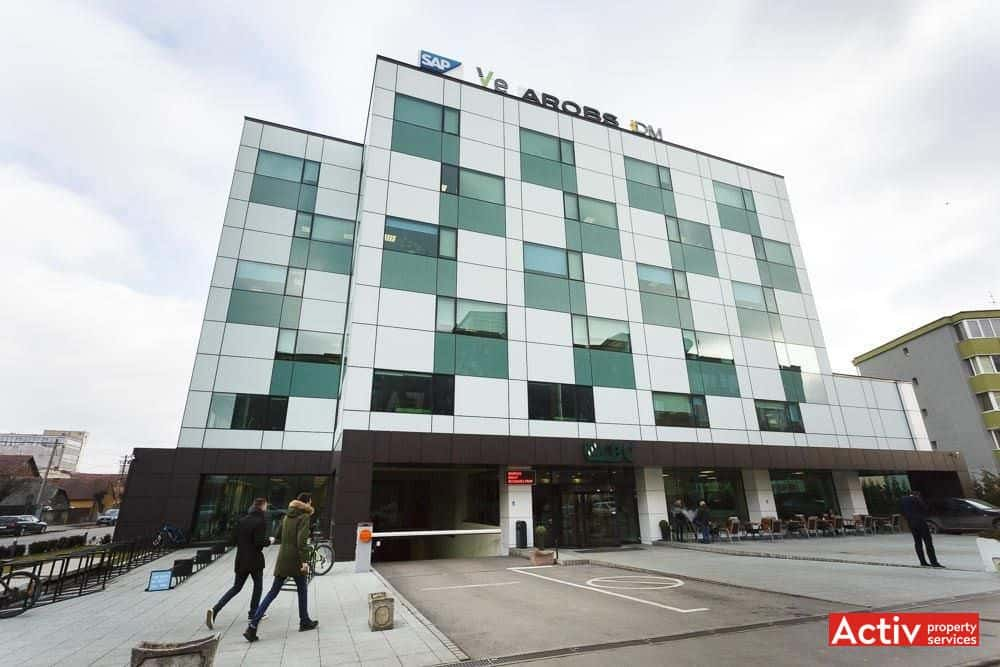
\includegraphics[width=0.75\textwidth, clip, trim=0cm 2cm 0cm 0cm]{cbc.jpg}

			\end{figuur}
			\vspace{-0.2ex}

			\noindent The primary office of AROBS is located in Cluj-Napoca, Romania. 
			It spans the second and third floor of the Cluj Business Center and houses a large part of the automotive department, consisting of over 400 employees.
			I spent most of my time working in the embedded department on the third floor of the building, where I was surrounded by friendly colleagues who were knowledgeable about anything from microcontrollers to FPGAs.
			
			Even though I was the only foreigner in the team, the atmosphere in the office was pleasant because I felt welcomed by my colleagues.
			They tried their best to speak English when I was around in order to include me in the conversation, which I really appreciated.
			My desk was next to a window with a beautiful view over the Baciu forest and its surrounding northern suburbs.
			A kitchen with the imperative coffee machine was just a small walk away from my desk.
			The business center also had facilities that I frequently made use of.
			Located on the first floor was a brunch restaurant from which a sweet smell emanated and filled the fitness center next to it.
			At the entrance was a coffee bar where I occasionally got my morning coffee.
			Once per month, a beer night was held to unite the department and encourage social activity among employees.
			I am left with the impression that AROBS is a modern company which invests in its employees by offering diverse activities.

			\noindent I was handed a laptop which I used for preparing documents and communicating with colleagues.
			Most internal communication at the company happened over Skype because it enabled inter-office messaging and helped to reach those who work at home.
			I was pleased with using Skype because I could instantly reach my company mentor and a few others who I was close with.
			It also allowed sending intermediate results during the development phase and getting feedback on them within a short timeframe.

			\vspace{1ex}
			\begin{figuur}{Organogram of AROBS Group}
				\centerline{
					\scalebox{0.9}{
				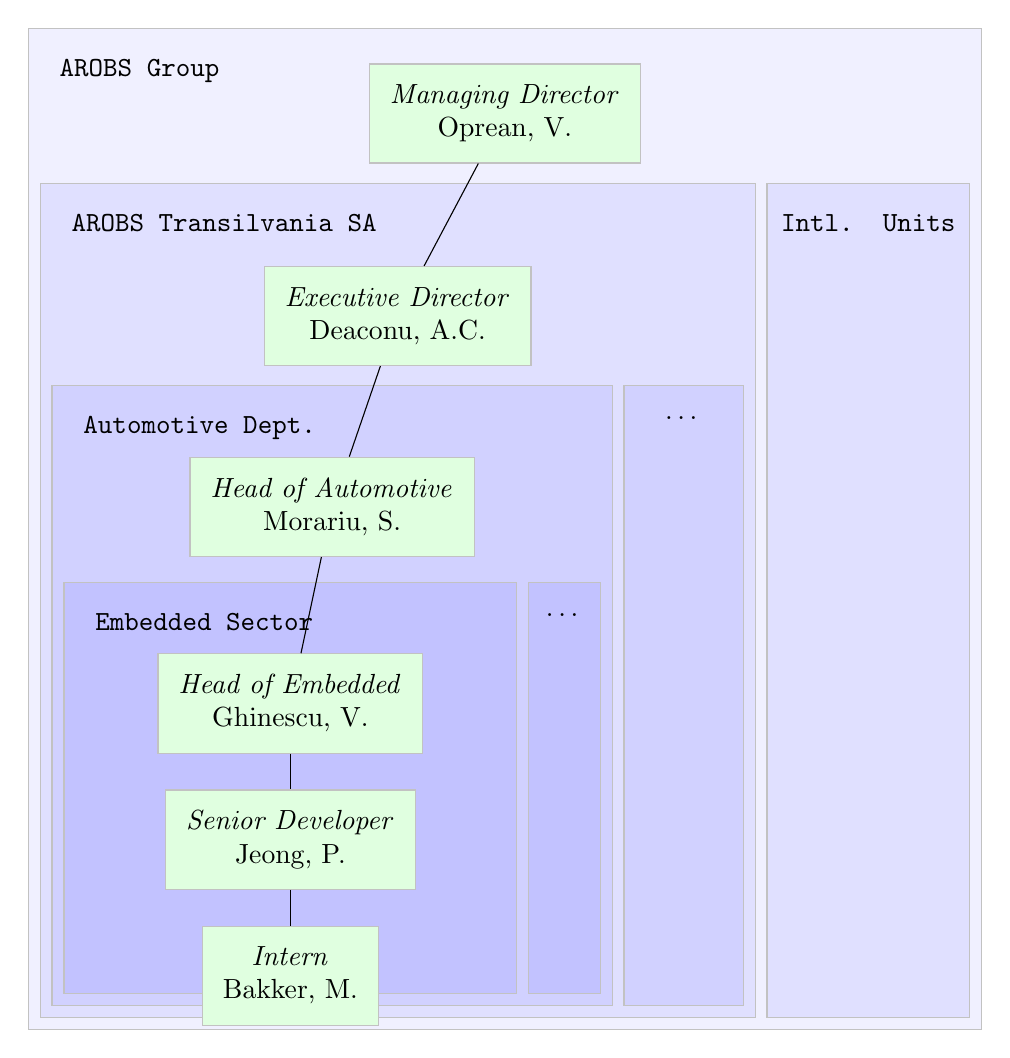
\begin{tikzpicture}
					
					\tikzstyle{grp}=[draw=black!24, align=right];
					\tikzstyle{man}=[draw=black!24, fill=green!12, align=center, inner sep=0.75em];

					\node (org) [grp, fill=blue!6, minimum width=80ex, minimum height=84ex, inner sep=0] {};
					\node (org label) [below right=0.8em and 0.8em of org.north west, align=left] {\ttfamily AROBS Group};
					\node (org man 1) [man, below=3ex of org.north] {\textit{Managing Director} \\ Oprean, V.};

					\node (rom) [grp, fill=blue!12, minimum width=60ex, minimum height=70ex, anchor=south west, above right=1ex and 1ex of org.south west, inner sep=0] {};
					\node (rom label) [below right=0.8em and 0.8em of rom.north west, align=left] {\ttfamily AROBS Transilvania SA};
					\node (rom man 1) [man, below=7ex of rom.north] {\textit{Executive Director} \\ Deaconu, A.C.};
					
					\node (oth) [grp, fill=blue!12, minimum width=17ex, minimum height=70ex, anchor=south east, above left=1ex and 1ex of org.south east, inner sep=0] {};
					\node (oth label) [below=0.8em of oth.north, align=center] {\ttfamily Intl. Units};

					\node (aum) [grp, fill=blue!18, minimum width=47ex, minimum height=52ex, anchor=south west, above right=1ex and 1ex of rom.south west, inner sep=0] {};
					\node (aum label) [below right=0.8em and 0.8em of aum.north west, align=left] {\ttfamily Automotive Dept.};
					\node (aum man 1) [man, below=6ex of aum.north] {\textit{Head of Automotive} \\ Morariu, S.};

					\node (otm) [grp, fill=blue!18, minimum width=10ex, minimum height=52ex, anchor=south east, above left=1ex and 1ex of rom.south east, inner sep=0] {};
					\node (otm label) [below=0.8em of otm.north, align=center] {\textellipsis};

					\node (emb) [grp, fill=blue!24, minimum width=38ex, minimum height=34.5ex, anchor=south west, above right=1ex and 1ex of aum.south west, inner sep=0] {};
					\node (emb label) [below right=0.8em and 0.8em of emb.north west, align=left] {\ttfamily Embedded Sector};
					\node (emb man 1) [man, below=6ex of emb.north] {\textit{Head of Embedded} \\ Ghinescu, V.};
					\node (emb man 2) [man, below=3ex of emb man 1.south] {\textit{Senior Developer} \\ Jeong, P.};
					\node (emb man 3) [man, below=3ex of emb man 2.south] {\textit{Intern} \\ Bakker, M.};
					
					\node (ots) [grp, fill=blue!24, minimum width=6ex, minimum height=34.5ex, anchor=south east, above left=1ex and 1ex of aum.south east, inner sep=0] {};
					\node (ots label) [below=0.8em of ots.north, align=center] {\textellipsis};

					\draw [-] (org man 1) -- (rom man 1);
					\draw [-] (rom man 1) -- (aum man 1);
					\draw [-] (aum man 1) -- (emb man 1);
					\draw [-] (emb man 1) -- (emb man 2);
					\draw [-] (emb man 2) -- (emb man 3);

				\end{tikzpicture}
					}
				}
			\end{figuur}
			\vspace{-0.2ex}

			\noindent I worked on the project alone, under the lead of my mentor.
			We talked multiple times per week when I had questions or new results to show.
			During the most critical phase of the project, the realization phase, we agreed to plan an additional meeting every Friday at 2 PM.
			These meetings allowed me to give updates on the development progress and any roadblocks I was facing.
			Other weeks were mostly spent on documentation and it was not worth holding a meeting because I would not have much news to show.

		\end{paragraaf}

		\begin{paragraaf}{The Project}

			One of AROBS' specialties is developing solutions for the automotive industry.
			Many of its clients have integrated the in-house developed Advanced Driver-Assistance System (ADAS) that aims to make cars more autonomous and relieve the driver of repetitive tasks.
			The value of automation in cars becomes clear when we view the statistics of road accidents: according to several studies \cite{nhtsa2017fatal} \cite{liu2009factors} \cite{dod2011run} conducted in the United States by the National Highway Traffic Safety Administration, \textit{human error} is the main factor in all fatal highway motorvehicle accidents.
			The study from 2016 shows that 94 percent of these were so-called "run-off-road crashes," which involved a single vehicle veering off the road and colliding with a natural or artificial object \cite{nhtsa2017fatal}.
			In these cases, the most common reason why the drivers lost control were intoxication and fatigue \cite{nhtsa2017fatal}.
			
			To take preventive measures against run-off-road crashes, the ADAS can be fitted with subsystems like a Lane Keeping System and a Lane Departure Warning System (LDWS).
			The latter is able to predict when a car is about to leave the lane and signal the ADAS of danger.
			Similarly to the stick shaker being activated in an aeroplane when it is about to stall, the car can notify the driver with a vibratory or auditory warning when it is unintentionally leaving the road lane.
			Other possible actions are automatically slowing down the car or correcting its course.

			In order to detect the position of the vehicle relative to the road lane, a video feed from the dashcam is processed by a computer vision algorithm.
			This algorithm is computationally expensive and requires to be run on an accelerated computing device like a Graphical Processing Unit (GPU.)
			Although lane detection systems using GPUs are widely used in prototypes and academic studies, they have failed to gain widespread adoption due to high production costs.
			Because GPUs are multipurpose devices that can be programmed to do many different tasks, they have been sought after by cryptocurrency miners, Machine Learning enthusiasts and big data hoarders, soaring the price up even higher.
			Since the start of the COVID-19 pandemic, the prices for GPUs have surged up to 150 percent of their list price due to factories not being able to produce them at full capacity \cite{cheng2021chip}.
			The increasing cost of these types of semiconductor devices has caused compaines like AROBS to consider replacing them with alternative hardware.
			
			Another device that can be programmed to process high amounts of data at once is a Field Programmable Gate Array.
			It is a chip that does not have a hardwired layout; it can be reconfigured to have different logic at any time.
			The chip is mass-produced in a "blank" state without any logic and the consumers can configure it to act like any digital logic circuit (as long as it fits on the chip's resources.)
			This means that an FPGA chip can be tailored to fit any use case.
			It also allows the FPGA designer fine-grained control over the chip's characteristics such as power draw and heat production.

			The core strength of an FPGA is parallel data processing.
			Digital logic circuits can be designed to have many signals that can work simultaneously, receiving the output of an operation on multiple data elements at the same time.
			In the field of image processing, this would mean that every pixel of an image could be processed simultaneously.
			A traditional processor would have to go over each pixel separately.

			I was assigned the task of creating an FPGA-based lane detection system that could outperform existing systems in terms of production cost per unit and power efficiency.
			With the market of hyper-autonomous cars being relatively new, this was a market opportunity that could have been seized.
			AROBS had previously built a GPU-based prototype system\,that was able detect road signs, objects and road lanes, which meant that there was a lot of knowledge in the company on the field of image processing.
			My mentor had worked on this prototype and was very knowledgeable on the subject of computer vision.
			With his help, it was my task to choose a sequence of algorithms that could be run on an FPGA and implement them in a proof-of-concept system.

			The initial situation was set out to be within the context of an existing vehicle.
			I assumed that systems for reading the dashcam footage and for propagating results to other ADAS subsystems for the car already existed.
			By placing them out of the scope of this project, I could focus my attention solely on developing the lane detector.

		\end{paragraaf}

		\begin{paragraaf}{Stakeholders}

			To make the project a success and meet the expectations of the parties who were involved with it, I had to make sure that each stakeholder's wishes would be satisfied.

			\vspace{2.5ex}
			\begin{figuur}{Stakeholder Analysis Matrix}
				\centerline{
				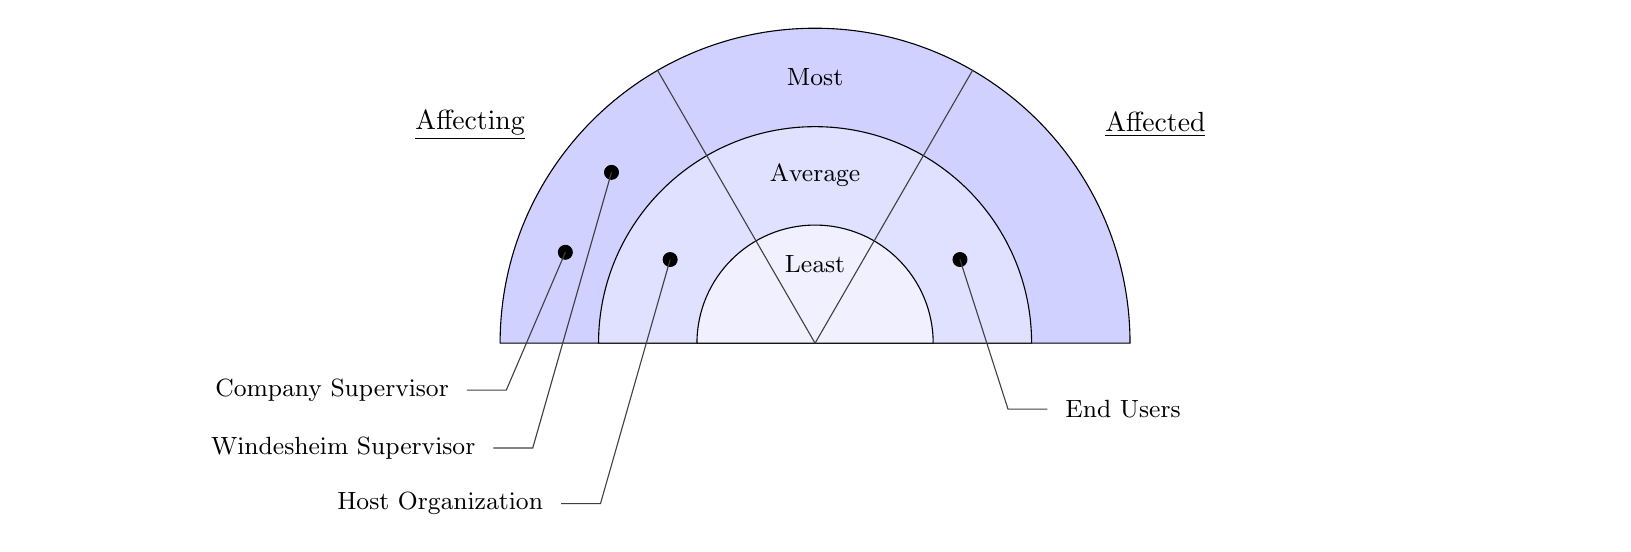
\begin{tikzpicture}[baseline=(current bounding box.north)]
					\path (-10, 0) -- (10, 0);
					\def\rad{4}
					\def\off{1.25}
					\def\offa{2.5}
					\draw [draw=black, fill=blue!18] (-\rad,0) -- (\rad,0) arc(0:180:\rad) --cycle;
					\draw [draw=black, fill=blue!12] (-\rad+\off,0) -- (\rad-\off,0) arc(0:180:\rad-\off) --cycle;
					\draw [draw=black, fill=blue!6] (-\rad+\offa,0) -- (\rad-\offa,0) arc(0:180:\rad-\offa) --cycle;
					%\draw [latex-latex] (-\rad, -0.5) -- (0, -0.5);
					\draw [color=darkgray] (0, 0) -- (60:\rad);
					\draw [color=darkgray] (0, 0) -- (120:\rad);

					\node[text centered] at (0, 1) {\small Least};
					\node[text centered] at (0, 2.125) {\small Average};
					\node[text centered] at (0, 3.375) {\small Most};
					\node[above right=2mm and 0.5cm of {(40:\rad)}, anchor=west] {\underline{Affected}};
					\node[above left=2mm and 0.5cm of {(140:\rad)}, anchor=east] {\underline{Affecting}};

					\coordinate (com sup p) at (160:\rad-\off/2);
					\coordinate (com sup s) at ($ (com sup p) + (-0.75, -1.75) $);
					\coordinate (com sup l) at ($ (com sup s) + (-0.5, 0) $);
					\filldraw (com sup p) circle (2.5pt);
					\draw [-, draw=darkgray] (com sup p)
						-- (com sup s)
						-- (com sup l);
					\node[left=0.7ex of com sup l, anchor=east] {\small Company Supervisor};

					\coordinate (win sup p) at (140:\rad-\off/2);
					\coordinate (win sup s) at ($ (win sup p) + (-1, -3.5) $);
					\coordinate (win sup l) at ($ (win sup s) + (-0.5, 0) $);
					\filldraw (win sup p) circle (2.5pt);
					\draw [-, draw=darkgray] (win sup p)
						-- (win sup s)
						-- (win sup l);
					\node[left=0.7ex of win sup l, anchor=east] {\small Windesheim Supervisor};

					\coordinate (host org p) at (150:\rad-\off-\off/2);
					\coordinate (host org s) at ($ (host org p) + (-0.885, -3.1) $);
					\coordinate (host org l) at ($ (host org s) + (-0.5, 0) $);
					\filldraw (host org p) circle (2.5pt);
					\draw [-, draw=darkgray] (host org p)
						-- (host org s)
						-- (host org l);
					\node[left=0.7ex of host org l, anchor=east] {\small Host Organization};
					
					\coordinate (end users p) at (30:\rad-\off-\off/2);
					\coordinate (end users s) at ($ (end users p) + (0.61, -1.9) $);
					\coordinate (end users l) at ($ (end users s) + (0.5, 0) $);
					\filldraw (end users p) circle (2.5pt);
					\draw [-, draw=darkgray] (end users p)
						-- (end users s)
						-- (end users l);
					\node[right=0.7ex of end users l, anchor=west] {\small End Users};

					%\draw [decorate, decoration={text along path, reverse path, raise=3ex, text={Affected}, text align={center}}] (\rad,0) arc(0:60:\rad);
					%\draw [decorate, decoration={text along path, raise=3ex, text={Affecting}, text align={center}}] (-\rad,0) arc(0:-60:-\rad);
				\end{tikzpicture}
				}
			\end{figuur}
			\vspace{-1ex}

			\noindent The above figure gives an overview of all stakeholders, along with their level of impact.
			It also shows whether a stakeholder has effect on the project or is affected by the outcome of the project.
			A brief description of each stakeholder and their interests is given in the following paragraphs.

			
			\begin{subparagraaf}{Host Organization}

				The organization instantiated this project and was the main driving force behind the resources of this project.
				It wanted to have evidence that FPGA-based technology could be used in this field by having a functional prototype.
				Although the organization was a secondary stakeholder, it could steer the project by giving the go/no go signal.
				It also purchased the hardware that I used to develop the system, which meant that it had financial resources invested and expected to see results from its investment.

			\end{subparagraaf}

			\begin{subparagraaf}{Company Supervisor}

				It was in the best interest of the company supervisor that I would deliver a working proof-of-concept system.
				Since the supervisor was my main point of contact within the company, I would be working with them closely, making them a high priority stakeholder.


			\end{subparagraaf}

			\begin{subparagraaf}{Windesheim Supervisor}

				This stakeholder was involved with giving approval of several deliverables, including the Plan of Action and the mid-term presentation.
				The main requirement set by this stakeholder was that the project was complex enough to be on par with level two of the HBO-ICT competences.
				I planned to comply with this by realizing complex products, such as implementing the image processing techniques and continuously testing the deliverables.
				They expected me to send a progress report at the end of every week for keeping watch on the status of my project.

			\end{subparagraaf}

			\begin{subparagraaf}{End Users}

				The system is abstracted away in the car, making it not directly accessible by the consumers.
				However, they will be relying on the system to give accurate results in order to guarantee their safety.
				Therefore, this stakeholder desires the system to be able to detect danger in real-time with low latency and high precision.

			\end{subparagraaf}

		\end{paragraaf}

	\end{hoofdstuk}
	
	\begin{hoofdstuk}{The Product}

		During the internship I created a prototype lane detector alongside tools that can interact with it.
		The lane detector itself is fully implemented on the TUL Z2 board.
		The tools are run on a personal computer or laptop that can be interfaced with it through a serial port.
		An example setup of the lane detector being interfaced with the Remote Control tool running on a mechanic's laptop can be seen in \verwijzingb{figuur}{Prototype Setup}.

		\begin{figuur}{Prototype Setup}
			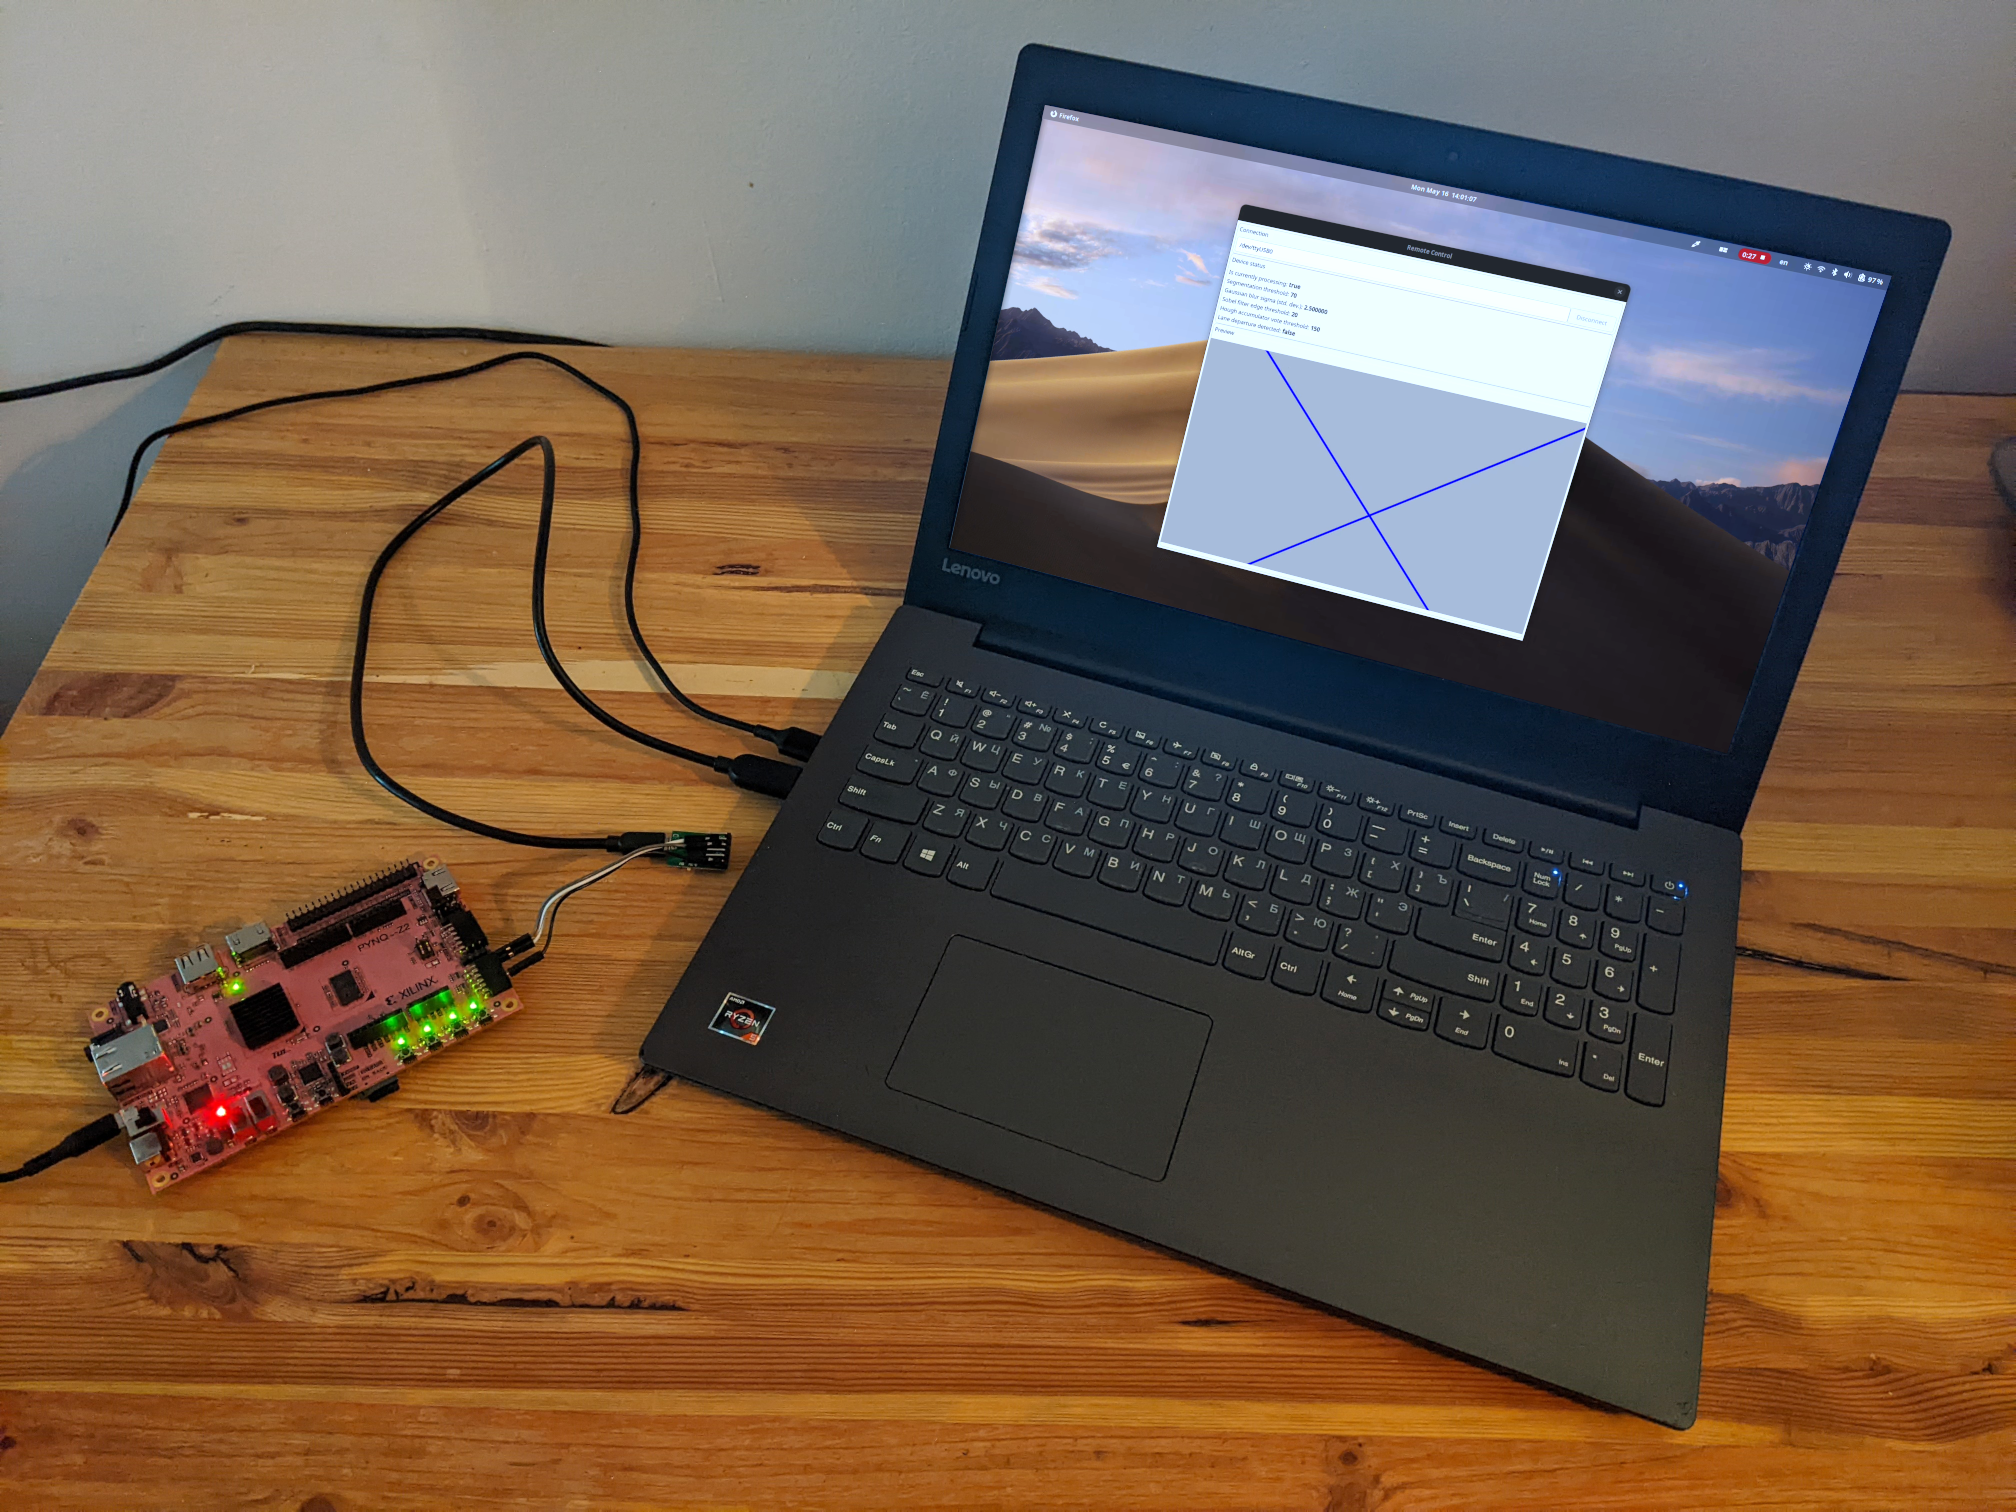
\includegraphics[width=0.8\textwidth]{product-5.png};
		\end{figuur}

		The total product can be distinguished into multiple deliverables that are able to be used together to form one functional system.
		An overview of this system is given in \verwijzingb{figuur}{Deliverables}.

		\begin{figuur}{Deliverables}
			\vspace{2ex}
			\centerline{
				\includegraphics{deliverables}
			}
		\end{figuur}

		\begin{paragraaf}{Lane Detector}

		\end{paragraaf}

		\begin{paragraaf}{Remote Control Application}

		\end{paragraaf}

		\begin{paragraaf}{Algorithm Toolsuite}

			I developed this application during the research phase of the project.
			It was my goal to get hands-on experience with the algorithms I researched by implementing them in a computer program.

		\end{paragraaf}

	\end{hoofdstuk}
	
	\begin{hoofdstuk}{Management and Control}

	\end{hoofdstuk}
	
	\begin{hoofdstuk}{Analyse}

	\end{hoofdstuk}
	
	\begin{hoofdstuk}{Advise}

	\end{hoofdstuk}
	
	\begin{hoofdstuk}{Design}

	\end{hoofdstuk}
	
	\begin{hoofdstuk}{Implementation}

	\end{hoofdstuk}
	
	\begin{hoofdstuk}{Professional Development}

	\end{hoofdstuk}

	% Bibliography page
	\begin{hoofdstuk}{References}

		\printbibliography[heading=none]

	\end{hoofdstuk}

	\makelastpage

\end{document}
